\section{$k$-clique Problem}

$k$-clique Problem belongs to $\NPC$ problems, its task is to decide whether there exists a clique with $k$ vertices in given graph $G$ with $n$ vertices. Note that there exists a $k$-clique in $G$ if and only if there exists a $k$-independent set in $\overline{G}$ if and only if there exists an $(n-k)$-vertex cover of $\overline{G}$ where $\overline{G}$ stands for complement to $G$.

For technical reasons we need $k$ to be even in all following examples; reduction from odd numbers will be solved in every single example.

Here if $k$ is odd, we add another vertex connected to every original vertex resulting in $G'$. Then existence of $(k+1)$-clique in $G'$ is equivalent to existence of $k$-clique in $G$. In following example in Figure \ref{fig:k-clique} we take $k$ even.

% reduction from SAT (wiki) ??

\subsection*{Set of tiles}

Here we describe tiles used by proposed DNA algorithm, Figure \ref{fig:k-clique} might be helpful. The amount of required tiles of given type will be given in terms of $n$ -- number of vertices, $e$ -- number of edges and $k$ -- size of seeked clique.

\begin{description}
	\item[Bottom tiles.] These tiles have colorless labels $2l$ and $2l-2$ $(0 < l \leq \frac{k}{2})$ on the bottom left and right sides, respectively. On the top sides there are numerically ordered\footnote{Later we will order by color. Note that this restriction does not reduce the set of candidate $k$-cliques.} numbers of vertices of all edges having $(k-2l+2)$-th and $(k-2l+1)$-th color, respectively. $e\cdot \frac{k}{2}$ tile types were required.
	\item[Bottom corner tiles.] These two tiles are connected on the bottom by the largest and the least colorless number, respectively. On the top they have a special glue: \# which can be viewed as $-\infty$ with respect to used ordering and * as $+\infty$, respectively. $2$ tile types were required.
	\item[Inner tiles.] These tiles are responsible for ordering\footnote{Principially they are the same as in Winfree \cite{winfree_phd}.} by color during which they verify existence of every edge. There exist all 2-color combinations of numbers of all connected vertices in both number-orders with both correct and reverse color-order on the bottom. On the top there are the same glues with correct color order. Moreover there exist similar tiles with sharp and asterisk instead of left or right number, respectively, with an exception: sharp and least color, and asterisk and largest color do not exist -- these are reserved for verification tiles. Remind that the top sharp or asterisk must have glue-strength equal to $2$.
	
	As soon as there appear numbers of unconnected vertices next to each other, the self assembly cannot continue and reach ``DONE'' because no tile can connect to this place. Note that colors were generated in reverse color order so they must meet each other during color ordering. Every missing edge would be revealed thus ``DONE'' tile connects if and only if the generated subset is a clique. $2\cdot\binom{k}{2}\cdot 2e + 2(k-1)n \sim 2 k^2 e + 2kn$ tile types were required.
	\item[Border tiles.] There are two tile types on the borders, one with sharps, one with asterisks. They just keep the structure growing up and signalize border. Remind that the bottom sharp or asterisk must have glue-strength $2$. $2$ tile types were required.
	\item[Verification tiles.] As soon as the least color reaches sharp and the largest color reaches asterisk there connect two special tiles which start verification whether nothing is missing. There exist two types of verification sequences ``C'' and ``D'' with all color--number combinations: ``D'' with the smaller half (by color), ``C'' with the higher half. $kn$ tile types were required.
	\item[DONE tile.] If everything is verified and verification sequences meet each other, ``DONE'' tile will be connected to signalize correct solution. $1$ tile type was required.
\end{description}

Summed up, tile complexity of this DNA algorithm is asymptotically equivalent to $2 k^2 e + 3 kn$. To compute Binding complexity easily we use following lemma.

\begin{lemma}
	In a square $\myatam$ tiling with $n$ bottom tiles, the number of bonds is asymptotically equivalent to $4 n^2$.
\end{lemma}
\begin{proof}
	Note that the square can be divided by diagonals into four triangles consisting of asymptotically $\frac{n^2}{2}$ tiles thus there are asymptotically $2n^2$ tiles. Every inner tile has four bonds, every inner bond belongs to two tiles thus there are asymptotically $4n^2$ bonds.
\end{proof}

Binding complexity is thus asymptotically equivalent to $\nicefrac{5}{4} \cdot 4 \bigl(\frac{k}{2}\bigr)^2 = \nicefrac{5}{4}\,k^2$, glue complexity is asymptotically equivalent to $kn$.

\begin{figure}[H]
\begin{center}
	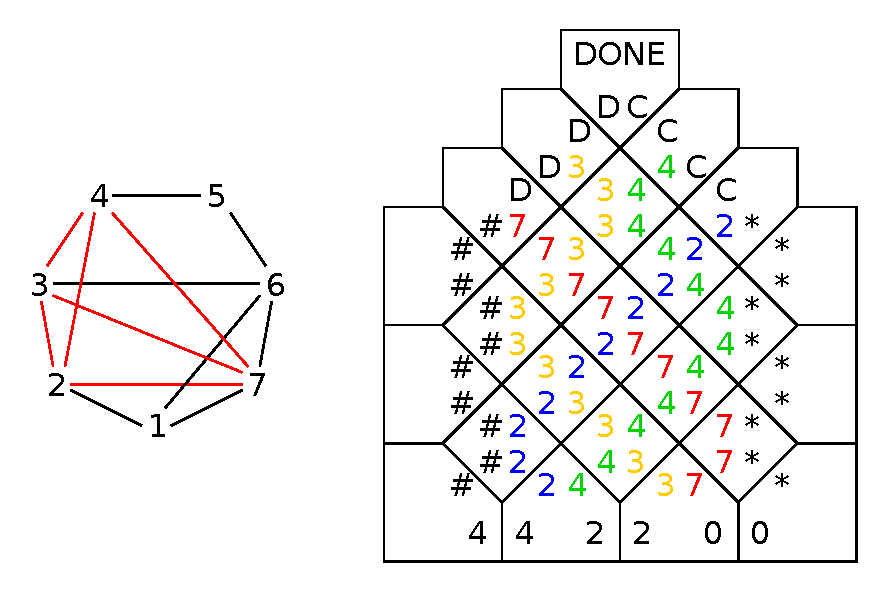
\includegraphics[scale=0.75]{./figures/k-clique/k-clique.pdf}
	\caption{$k$-clique computation. Color order is defined by the wavelength of the colors.}
	\label{fig:k-clique}
\end{center}
\end{figure}

\subsection{Simulation in {\tt xgrow}}

{\tt xgrow} is an open source DNA tile assembly simulator written by Erik Winfree, Rebecca Schulman and Constantine Evans. It is freely available at \url{www.dna.caltech.edu/Xgrow}. It is capable of both $\atam$ and $\ktam$ simulations.

{\tt xgrow} takes some settings and a file with tiles on input, then it conducts a simulation. We used {\tt xgrow} to verify our algorithm for $k$-clique Problem so we wrote a script which generates input file with tiles for {\tt xgrow}. The script is called {\tt k-clique.rb}, it is written in Ruby language and it is provided on attached CD.

\subsubsection*{Running a simulation}

Though everything is cross-platform, this paragraph describes how to run a simulation under Linux systems. You need to download and compile {\tt xgrow} and install Ruby interpreter. Then you need to generate an input graph representation. Open Terminal in your directory with {\tt k-clique.rb} and run {\tt irb} which is an interactive Ruby shell. Then run following commands:
\begin{verbatim}
require "yaml"
# replace by your graph's adjacency matrix written
# as array of lines (upper triangle suffices):
graph = [[0, 1, 0], [0, 0, 1], [0, 0, 0]]
# define output file
f = File.open("graph.yaml", "w")
# dump graph into yaml, write to file
f.write(YAML.dump(graph))
f.close
exit
\end{verbatim}
Your graph is now stored in {\tt graph.yaml}. Now run {\tt k-clique.rb} in your directory with two parameters: first parameter is $k$ -- size of clique, second parameter is filename with your graph, and redirect output to a new {\tt *.tiles} file, e.g. {\tt ./k-clique.rb 4 graph.yaml > 4-clique.tiles}. Then move {\tt 4-clique.tiles} file to {\tt xgrow-install-dir/tilesets/4-clique.tiles} and run an $\atam$ simulation by {\tt ./xgrow 4-clique T=2} or a $\ktam$ simulation by {\tt ./xgrow 4-clique}.

Note that {\tt xgrow} performs a probabilistic simulation thus accepting tile\footnote{In our script the accepting tile is magenta.} can appear very unlikely (depends on probability of random choosing a $k$-clique in your graph). So if you want to see accepting computation you need to set probabilities of tiles which generate our clique to a reasonably high value. These probabilities can be set in your {\tt *.tiles} file in a block {\tt tile edges}, on every line there is a number in square brackets which represents relative concentration which is proportional to probability. A sample output for $\atam$ simulation can be seen in Figure \ref{fig:xgrow}.

\begin{figure}[h]
\begin{center}
	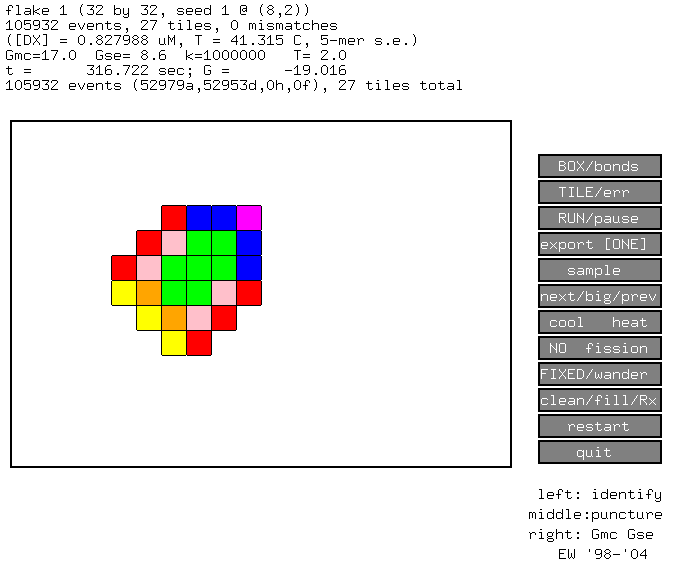
\includegraphics[scale=0.55]{./figures/xgrow/xgrow.png}
	\caption{$k$-clique computation simulated by {\tt xgrow} with $\atam$. Magenta tile represents DONE tile.}
	\label{fig:xgrow}
\end{center}
\end{figure}

Running a $\ktam$ simulation in {\tt xgrow} leads to very unstable evolution process with many errors, it is very hard (but not impossible) to reach DONE tile. The only possibility to get a flake without errors is slow annealing which can be regulated by {\tt cool heat} button.